\chapter{Results}
\thispagestyle{empty}

    Experiments show that the both SegAN and MultiResUNet achieved almost the same dice coefficient result for the noise free images
    but vanilla U-Net did not achieved similar results in terms of the same similarity metrics. It's not as successful as the others.
    MultiResUNet is slightly more successful than SegAN if they compared with Jaccard coefficient.
    The detailed results are given in the Table ~\ref{table:all-metrics-all-noises-unet}, ~\ref{table:all-metrics-all-noises-segan} and ~\ref{table:all-metrics-all-noises-multiresunet} through statistical metrics.
    Although the dice results of MultiResUNet and SegAN are very close for the noiseless datasets, the dice results differ for the all models as the noise level increases.

    Both MultiResUnet and SegAN achieved their best results around the epoch size of 50. The results were found similar after this point.
    Figure ~\ref{figure:all-noises-by-epoch-dice-unet}, ~\ref{figure:all-noises-by-epoch-dice-multiresunet} and ~\ref{figure:all-noises-by-epoch-dice-segan} point out the dice results of models at different levels of epoch size.
    Figure ~\ref{figure:segan-avg-dice}, ~\ref{figure:segan-bad-dice} and ~\ref{figure:segan-good-dice} show the evaluation results of dermoscopic images from the evaluation dataset with different success rates.
    Furthermore, Figure ~\ref{figure:multiresunet-avg-dice}, ~\ref{figure:multiresunet-bad-dice} and ~\ref{figure:multiresunet-good-dice} show the results of MultiResUNet with different success rates.

    \sidebyside
        {05-results/figures/segan/avg/ISIC_0012330.jpg}{Original image}
        {05-results/figures/segan/avg/ISIC_0012330.png}{Ground truth}
        {05-results/figures/segan/avg/ISIC_0012330_dice_8288.png}{Result(dice=0.82)}
        {SegAN result with average score at 0\% of Gaussian noise}{figure:segan-avg-dice}

    \sidebyside
        {05-results/figures/segan/bad/ISIC_0012136.jpg}{Original image}
        {05-results/figures/segan/bad/ISIC_0012136.png}{Ground truth}
        {05-results/figures/segan/bad/ISIC_0012136_dice_5015.png}{Result(dice=0.50)}
        {SegAN result with low success compared to average at 0\% of Gaussian noise}{figure:segan-bad-dice}

    \sidebyside
        {05-results/figures/segan/good/ISIC_0012152.jpg}{Original image}
        {05-results/figures/segan/good/ISIC_0012152.png}{Ground truth}
        {05-results/figures/segan/good/ISIC_0012152_dice_9112.png}{Result(dice=0.91)}
        {SegAN result with high success compared to average at 0\% of Gaussian noise}{figure:segan-good-dice}

    \sidebyside
        {05-results/figures/multiresunet/avg/ISIC_0012152.jpg}{Original image}
        {05-results/figures/multiresunet/avg/ISIC_0012152.png}{Ground truth}
        {05-results/figures/multiresunet/avg/ISIC_0012152_dice_8048.jpg}{Result(dice=0.80)}
        {MultiResUNet result with average score at 0\% of Gaussian noise}{figure:multiresunet-avg-dice}

    \sidebyside
        {05-results/figures/multiresunet/bad/ISIC_0012356.jpg}{Original image}
        {05-results/figures/multiresunet/bad/ISIC_0012356.png}{Ground truth}
        {05-results/figures/multiresunet/bad/ISIC_0012356_dice_543.jpg}{Result(dice=0.54)}
        {MultiResUNet result with low success compared to average at 0\% of Gaussian noise}{figure:multiresunet-bad-dice}

    \sidebyside
        {05-results/figures/multiresunet/good/ISIC_0012092.jpg}{Original image}
        {05-results/figures/multiresunet/good/ISIC_0012092.png}{Ground truth}
        {05-results/figures/multiresunet/good/ISIC_0012092_dice_904.jpg}{Result(dice=0.90)}
        {MultiResUNet result with high success compared to average at 0\% of Gaussian noise}{figure:multiresunet-good-dice}

    When the noise level is 50\%, the dice results of MultiResUNet's decreased up to 28\%, the U-Net's decreased up to 23\%, while the SegAN's decreased up to 53\%.
    As it explained in Section ~\ref{section:multiresunet}, SegAN introduces fake skin lesions during the generator level and the discriminator
    takes a decision after the training if test image is a lesion.
    The noise added during the training phase of SegAN makes the model more successful against noisy data.

    Figure ~\ref{figure:comparision-of-models-for-noise-tolerance} shows the change of success of the models against noise.
    As can be seen here, SegAN is more robust than vanilla U-Net and MultiResUNet at increased levels of Gaussian noises.

    \begin{figure}
    \centerline{\scalebox{0.55}{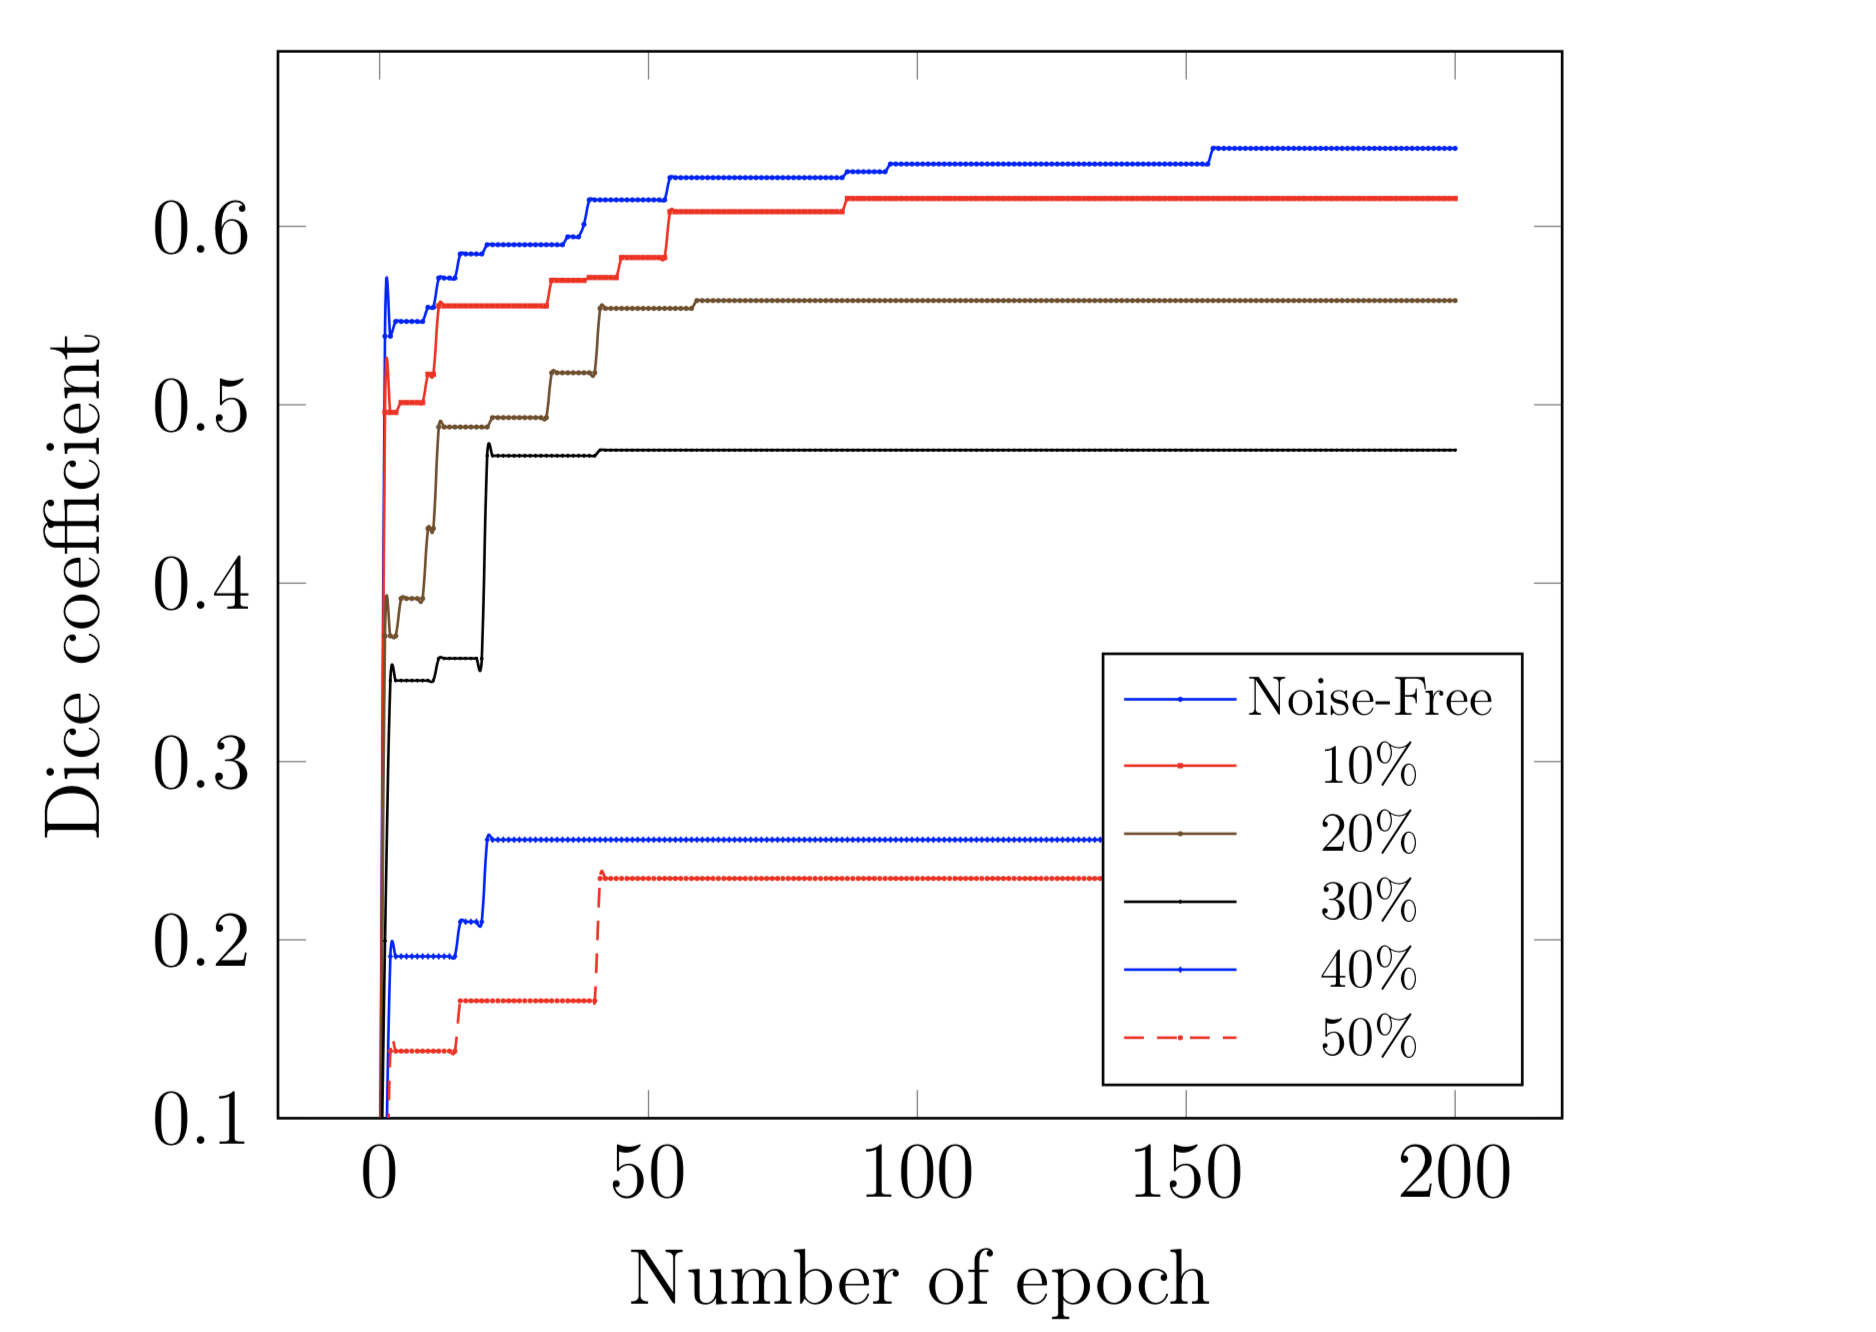
\includegraphics{05-results/figures/all-noises-by-epoch-dice-unet.png}}}
    \caption{Dice results for U-Net at different Gaussian noises by number of epochs}
    \label{fig:all-noises-by-epoch-dice-unet}
\end{figure}

%\figureallnoises
%    {05-results/plots/all-noises-by-epoch-dice-multiresunet.txt}
%    {Dice results for MultiResUNet at different Gaussian noises by number of epochs}
%    {fig:all-noises-by-epoch-dice-multiresunet}

    \begin{figure}
    \centerline{\scalebox{0.55}{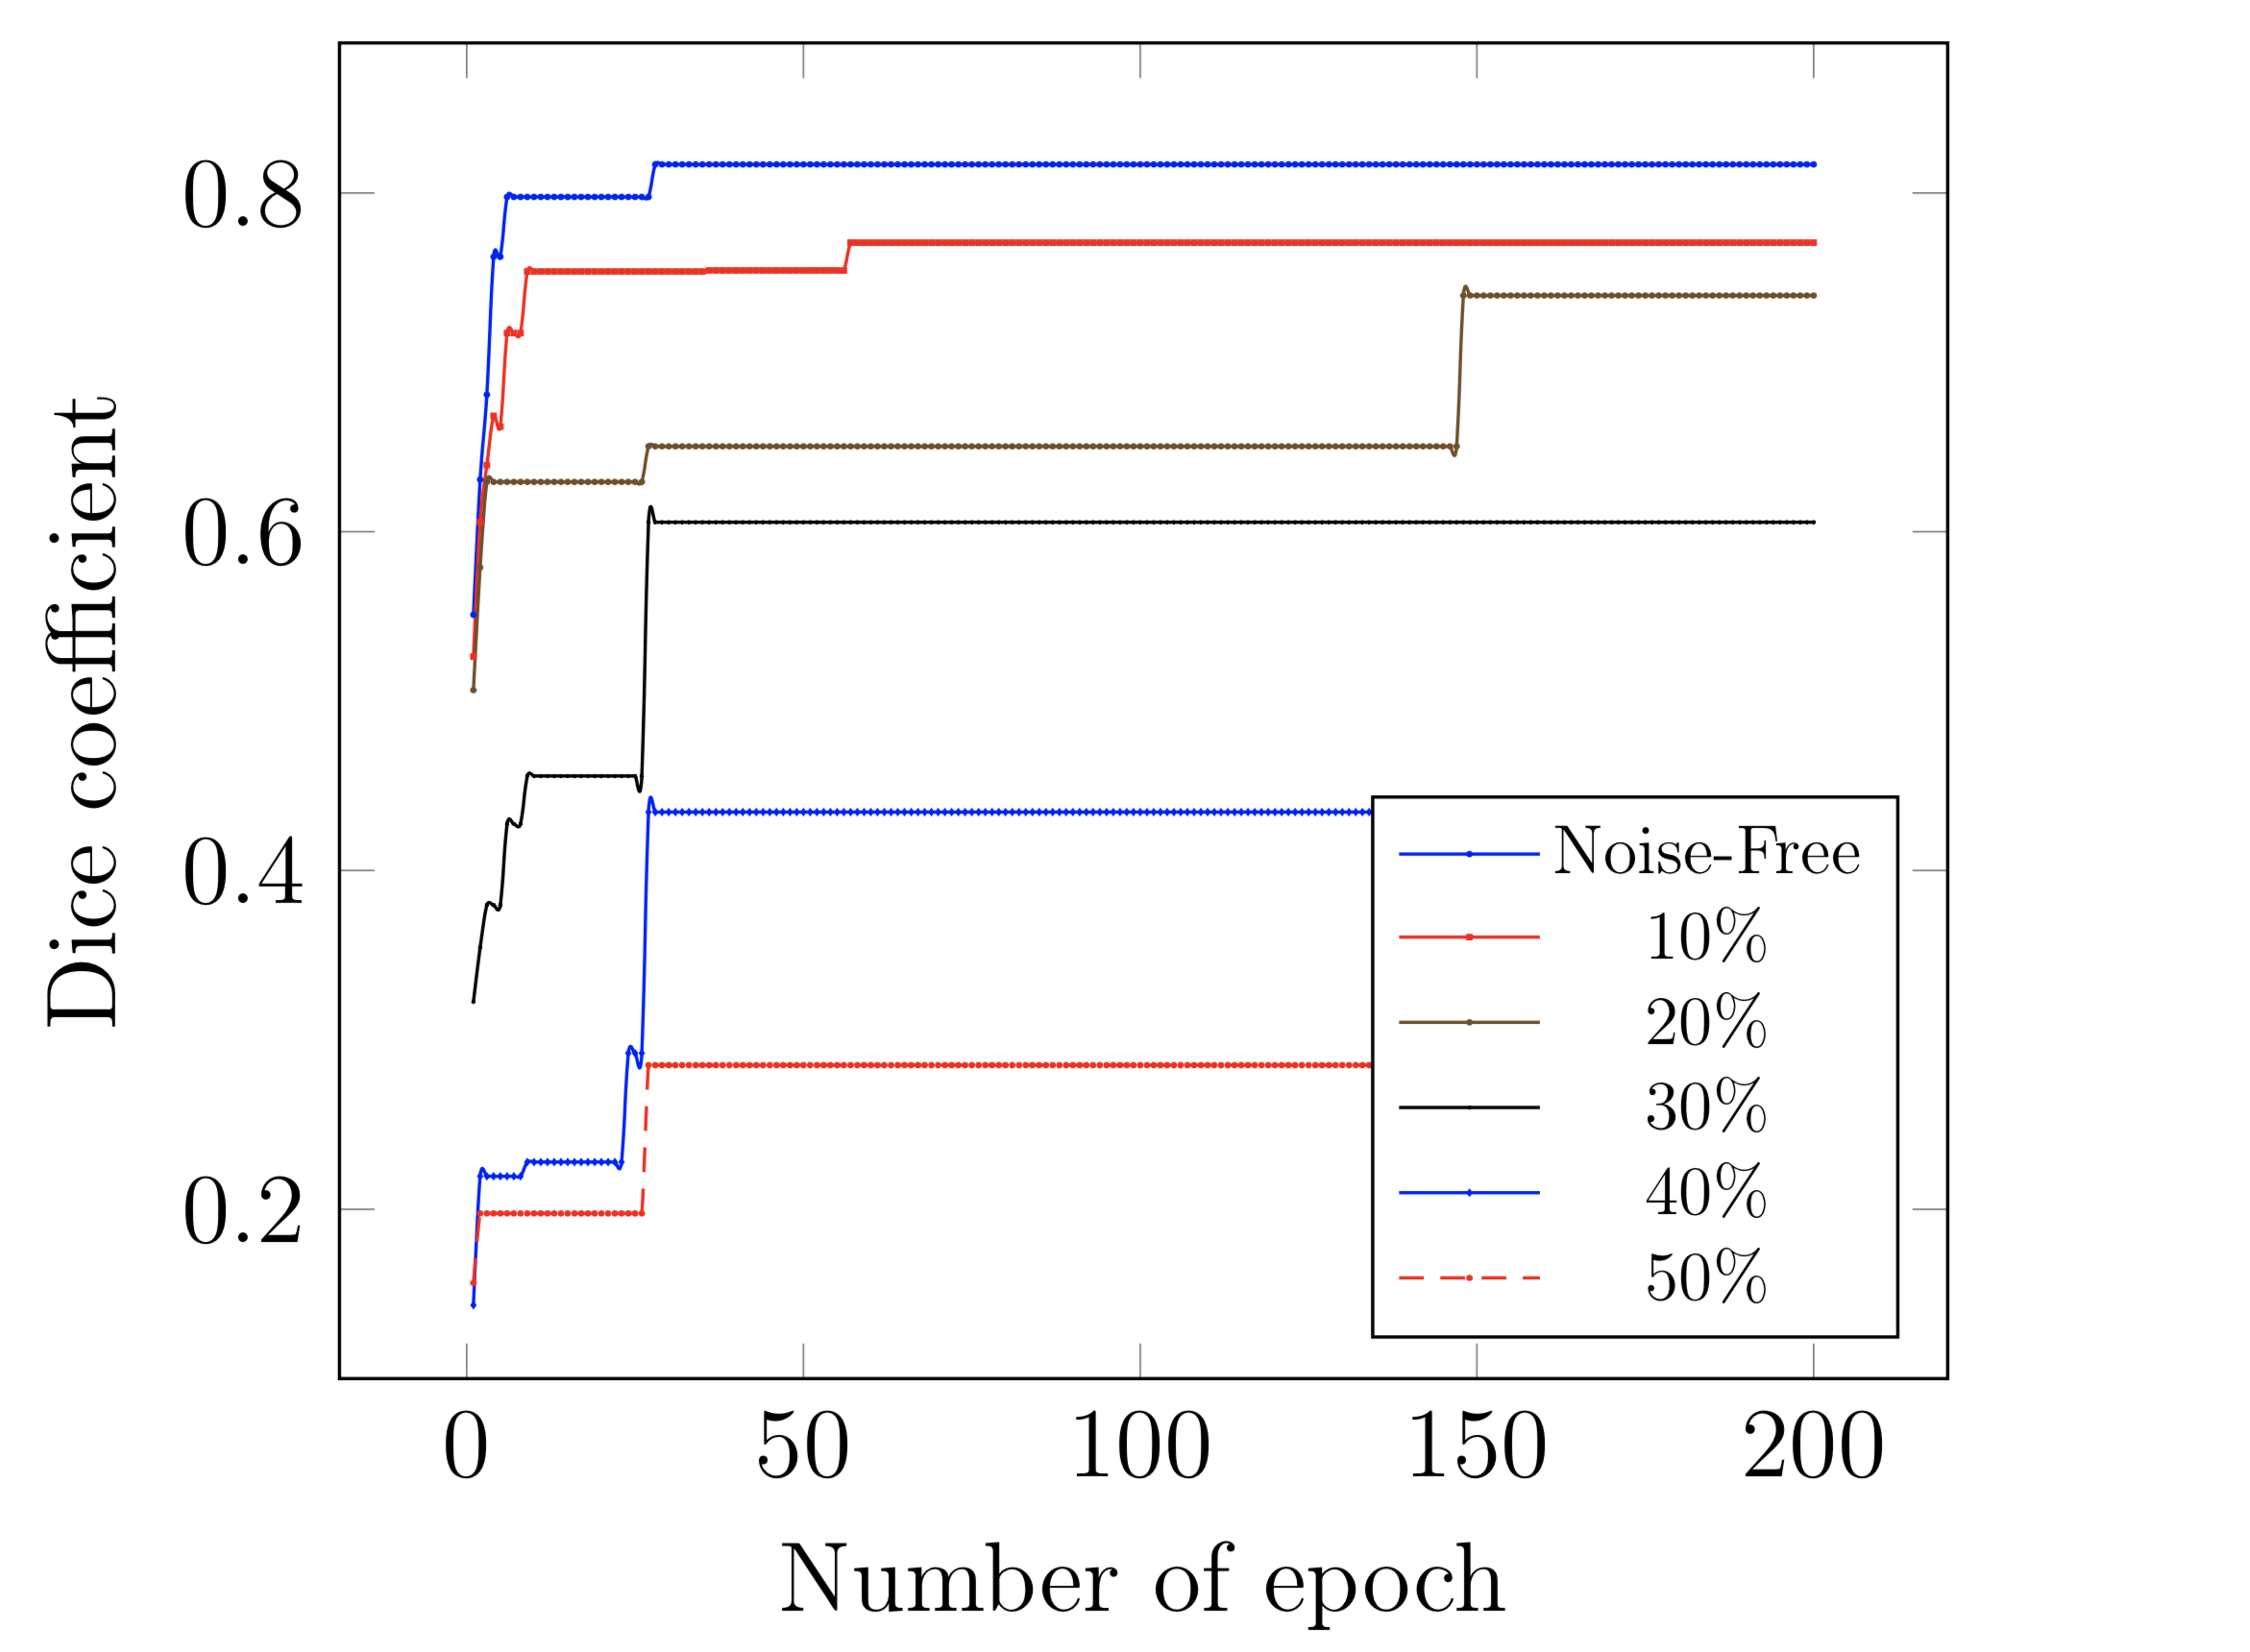
\includegraphics{05-results/figures/all-noises-by-epoch-dice-segan.png}}}
    \caption{Dice results for SegAN at different Gaussian noises by number of epochs}
    \label{fig:all-noises-by-epoch-dice-segan}
\end{figure}

%\figureallnoises
%    {05-results/plots/all-noises-by-epoch-dice-segan.txt}
%    {Dice results for SegAN at different Gaussian noises by number of epochs}
%    {fig:all-noises-by-epoch-dice-segan}


    \begin{figure}
    \centerline{\scalebox{0.55}{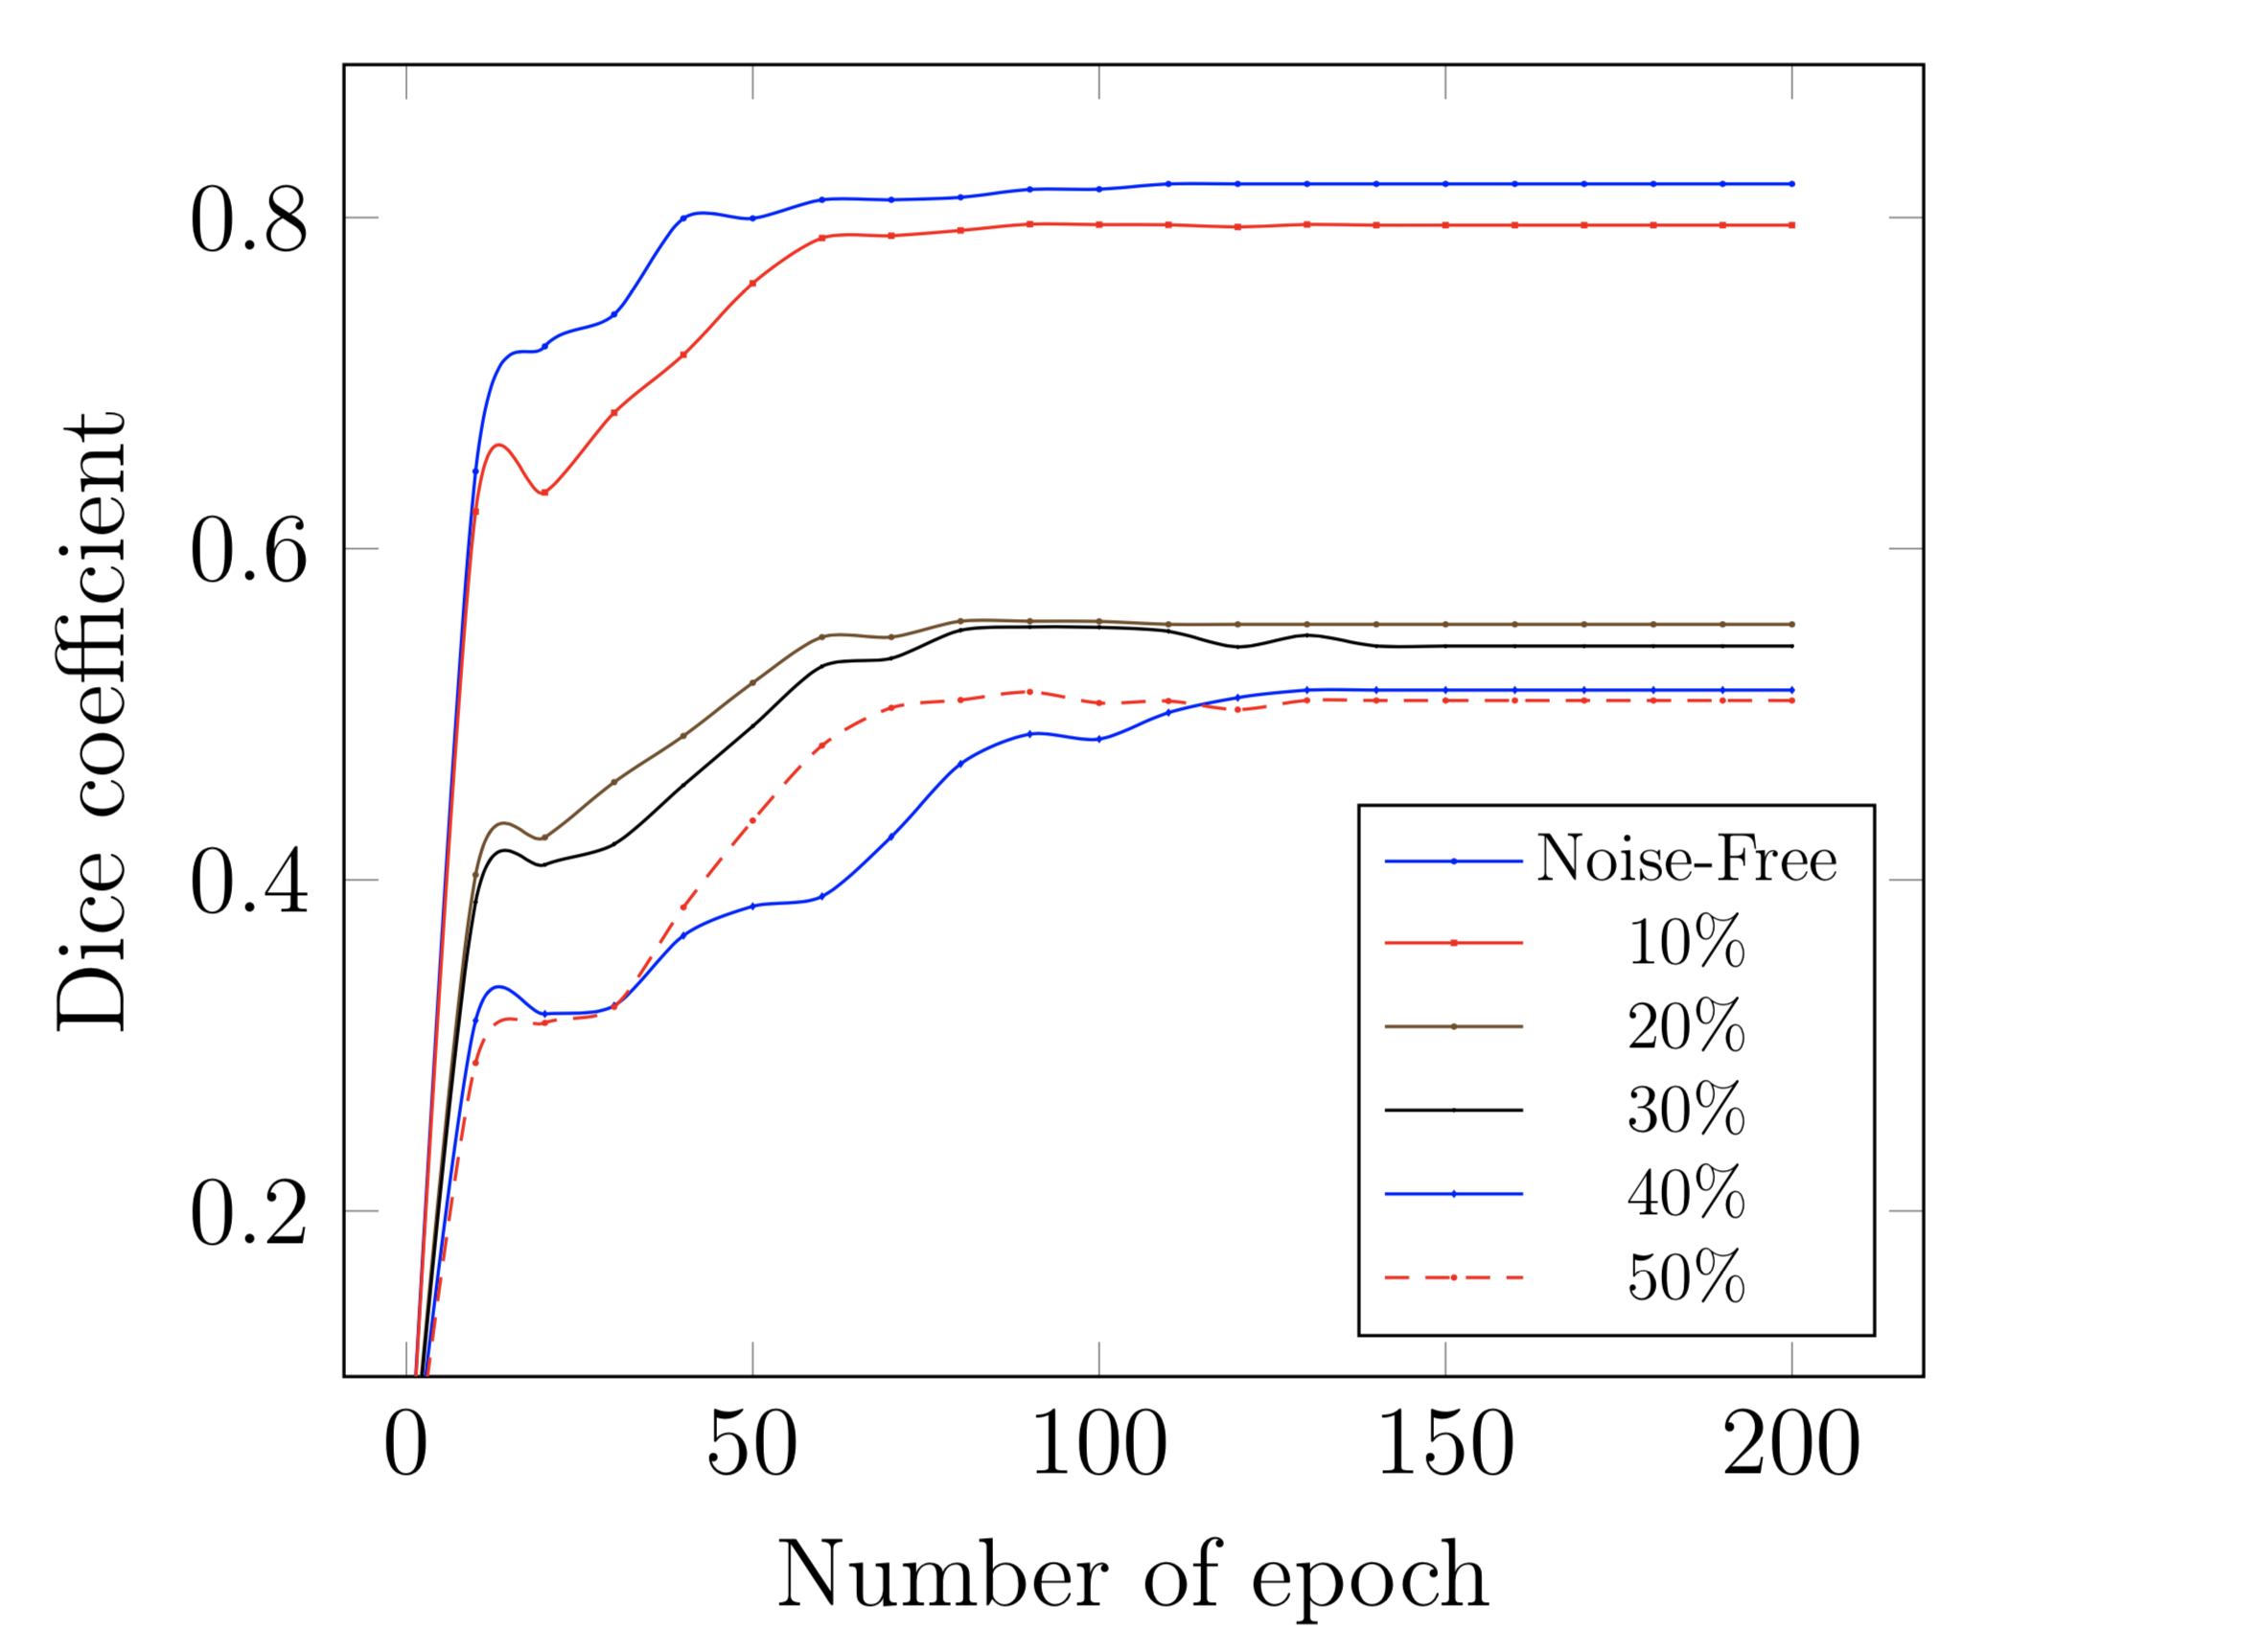
\includegraphics{05-results/figures/all-noises-by-epoch-dice-multiresunet.png}}}
    \caption{Dice results for MultiResUNet at different Gaussian noises by number of epochs}
    \label{fig:all-noises-by-epoch-dice-multiresunet}
\end{figure}

%\figureallnoises
%    {05-results/plots/all-noises-by-epoch-dice-multiresunet.txt}
%    {Dice results for MultiResUNet at different Gaussian noises by number of epochs}
%    {fig:all-noises-by-epoch-dice-multiresunet}

    \begin{table}[h]
\caption{Comparision of segmentation results of U-Net at different levels of Gaussian noise with evaluation metrics}
\centering
\begin{tabular}{c|ccccc}
Gaussian noise(\%)   & Dice   & Jaccard & Accuracy & Sensitivity & Specificity \\
\specialrule{2pt}{1pt}{1pt}
0  & 0.6437 & 0.5343 & 0.8619 & 0.7350 & 0.8825 \\
10 & 0.6156 & 0.5087 & 0.8559 & 0.7562 & 0.8718 \\
20 & 0.5584 & 0.4482 & 0.8423 & 0.7680 & 0.8507 \\
30 & 0.4746 & 0.3707 & 0.8282 & 0.7817 & 0.8316 \\
40 & 0.2562 & 0.1737 & 0.7853 & 0.6236 & 0.7941 \\
50 & 0.2345 & 0.1638 & 0.7954 & 0.7575 & 0.7869 \\
\hline
\end{tabular}
\label{table:all-metrics-all-noises-unet}
\end{table}


    \begin{table}[h]
\caption{Comparision of segmentation results of SegAN at different levels of Gaussian noise with evaluation metrics}
\centering
\begin{tabular}{c|ccccc}
Gaussian noise(\%)   & Dice   & Jaccard & Accuracy & Sensitivity & Specificity \\
\specialrule{2pt}{1pt}{1pt}
0   & 0.8110   & 0.6968  & 0.9236 & 0.8998 & 0.9240      \\
10  & 0.5570   & 0.4     & 0.8129 & 0.6232 & 0.8445      \\
20  & 0.5518   & 0.3936  & 0.8134 & 0.6322 & 0.8417      \\
30  & 0.5456   & 0.3878  & 0.8132 & 0.6329 & 0.8398      \\
40  & 0.5378   & 0.3791  & 0.809  & 0.6085 & 0.8442      \\
50  & 0.5368   & 0.3783  & 0.8115 & 0.6364 & 0.8351      \\
\hline
\end{tabular}
\label{all-metrics-all-noises-segan}
\end{table}

    \begin{table}[h]
\caption{Comparision of segmentation results of MultiResUNet at different levels of Gaussian noise with evaluation metrics}
\centering
\begin{tabular}{c|ccccc}
Gaussian noise(\%)   & Dice   & Jaccard & Accuracy & Sensitivity & Specificity \\
\specialrule{2pt}{1pt}{1pt}
0  & 0.8169 & 0.7221 & 0.922  & 0.964  & 0.9482 \\
10 & 0.7707 & 0.6747 & 0.9058 & 0.8923 & 0.9024 \\
20 & 0.7395 & 0.624 & 0.8829 & 0.8788 & 0.8705 \\
30 & 0.6056 & 0.4784 & 0.6056 & 0.8402 & 0.7949 \\
40 & 0.4345 & 0.3061   & 0.8062 & 0.7033 & 0.8104 \\
50 & 0.2851 & 0.1969 & 0.7878 & 0.7729 & 0.7847 \\
\hline
\end{tabular}
\label{all-metrics-all-noises-multiresunet}
\end{table}

    \begin{figure}
    \centerline{\scalebox{0.55}{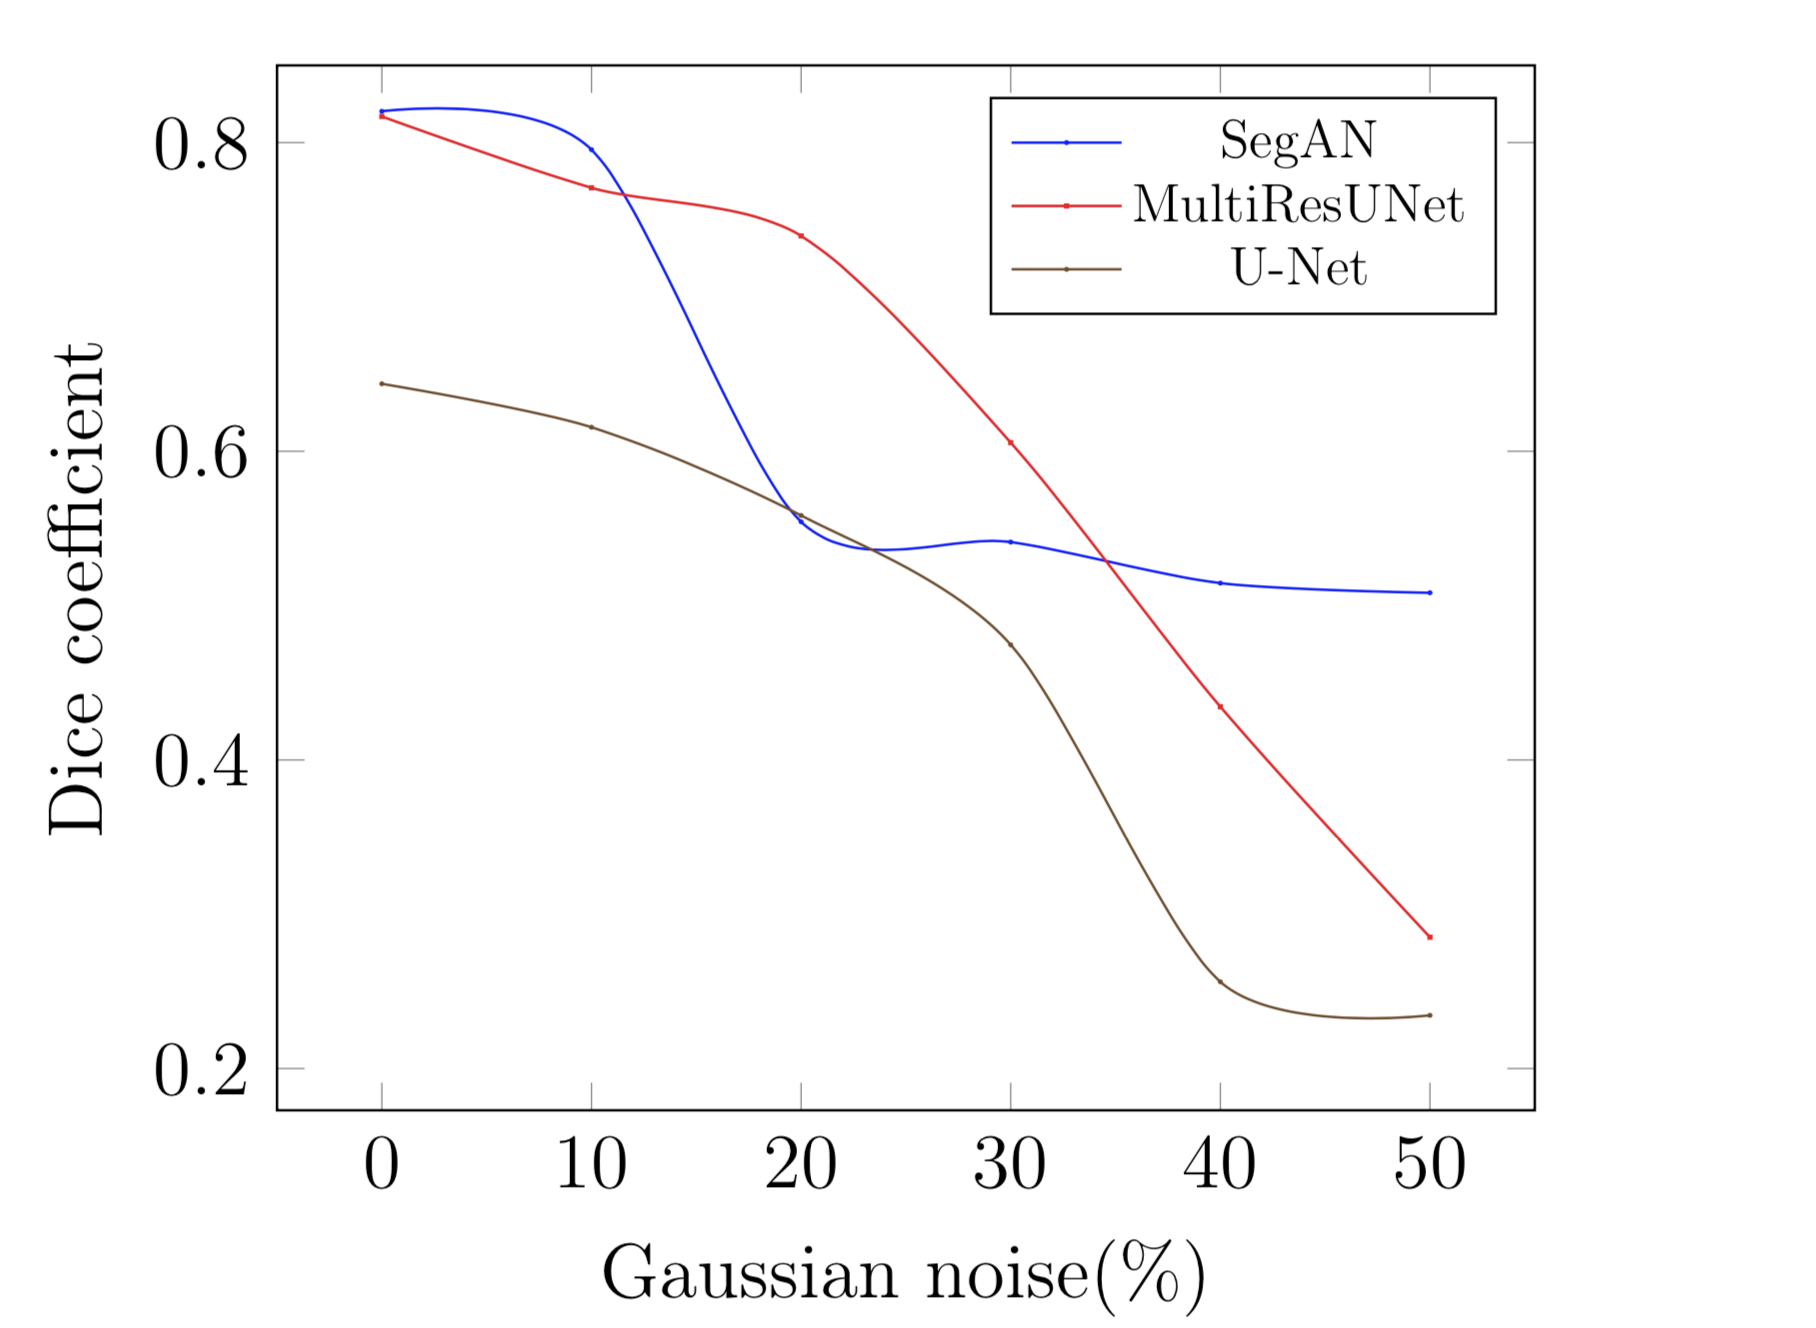
\includegraphics{05-results/figures/comparision-of-results-of-models-at-different-noise-levels.png}}}
    \caption{Comparision of the results of the models at different noise levels}
    \label{fig:comparision-of-results-of-models-at-different-noise-levels}
\end{figure}

%\figureavgnoises
%    {05-results/plots/dice-scores-with-different-gaussian-noise.csv}
%    {Dice result for SegAN at different Gaussian noises}
%    {fig:noise-tolerance-dice-segand}


    \begin{figure}
    \centerline{\scalebox{0.55}{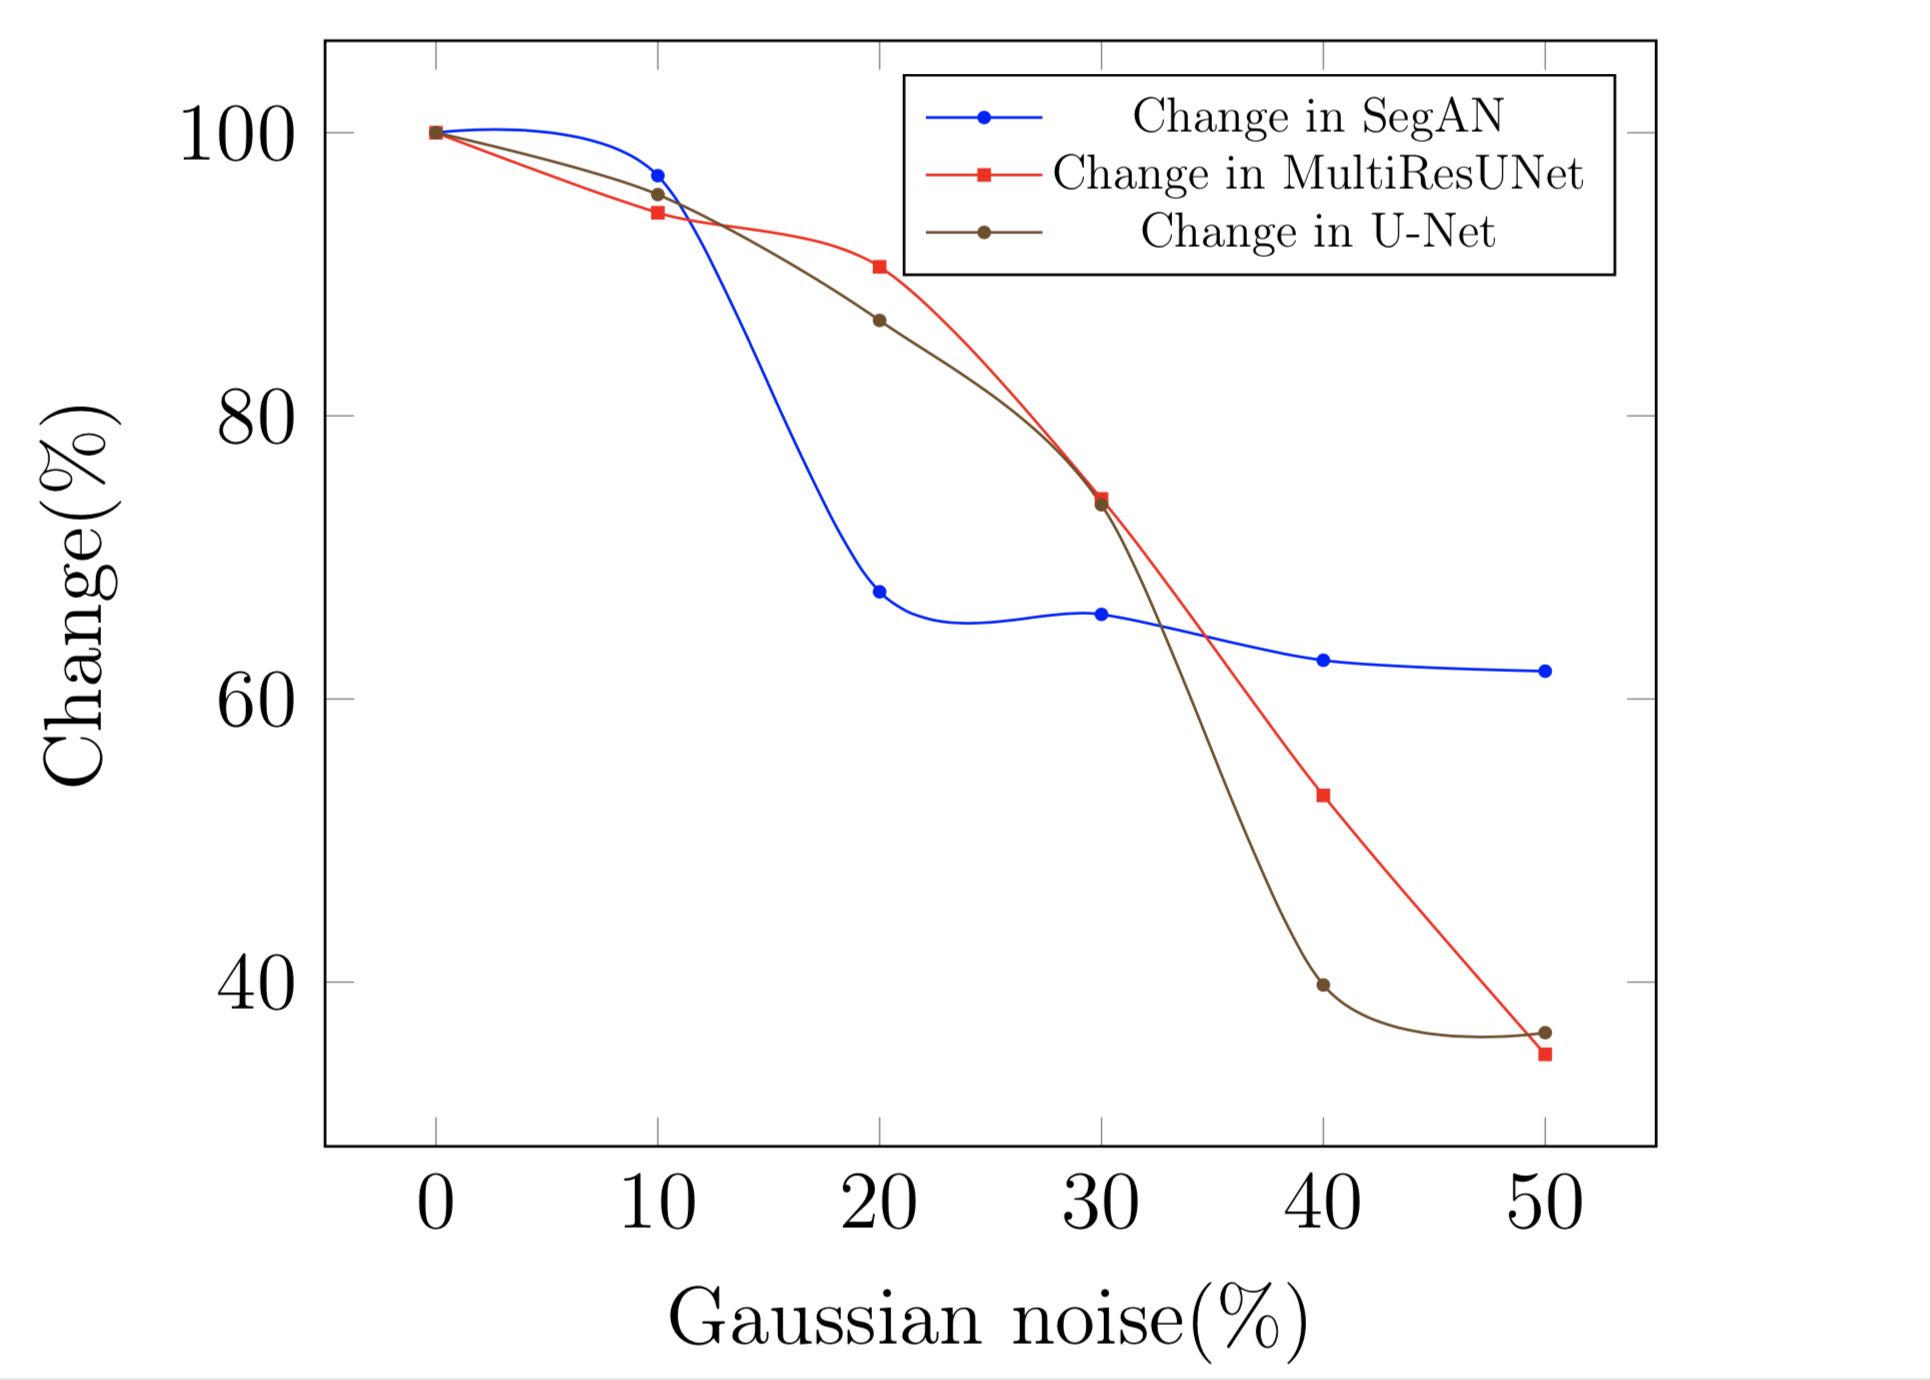
\includegraphics{05-results/figures/comparision-of-models-for-noise-tolerance.png}}}
    \caption{Change of success of the models by noise level}
    \label{fig:comparision-of-models-for-noise-tolerance}
\end{figure}

%\figuretolerancenoises
%    {04-methodology/plots/dice-scores-with-different-gaussian-noise.csv}
%    {Change of success of the models by noise level}
%    {fig:noise-tolerance-dice-seganda}

    \begin{figure}
    \centerline{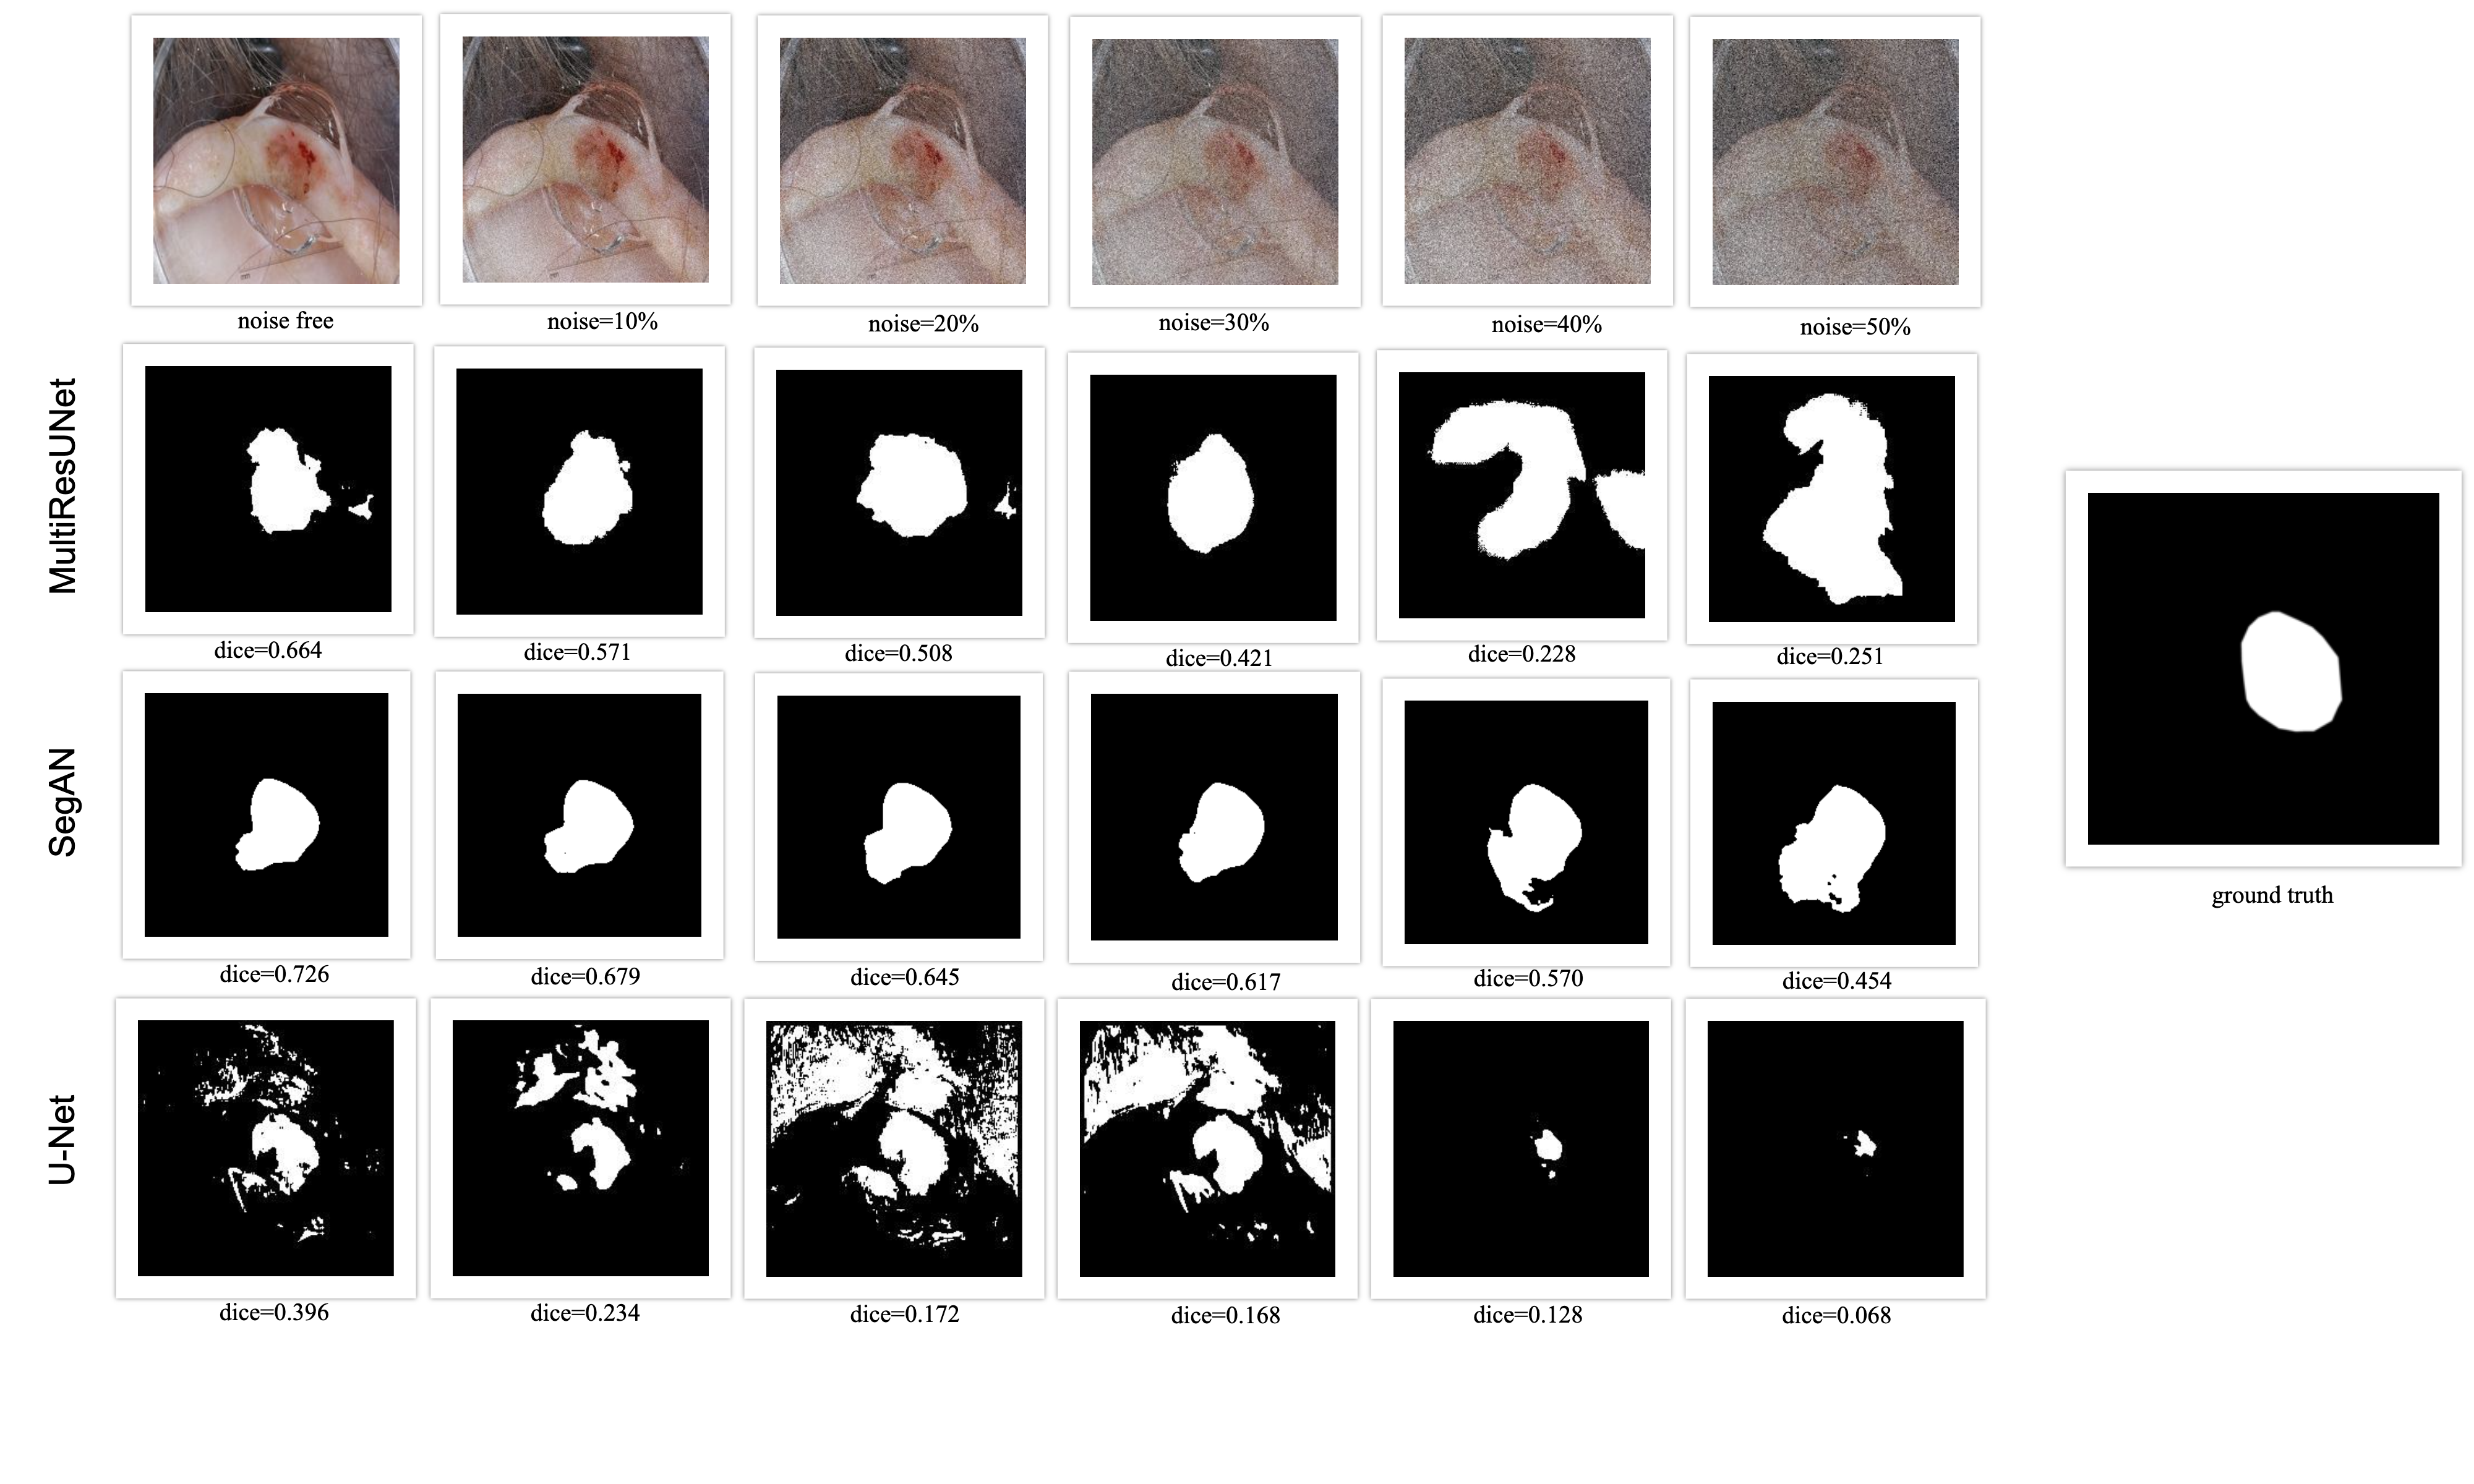
\includegraphics[width=1\columnwidth]{05-results/figures/extended_results_sample_gan_over_unet.png}}
    \caption{Dice results of the same image for SegAN and MultiResUNet at different Gaussian noises. The images in a column from top to bottom show the input, MultiResUnet result and SegAN result respectively. SegAN has better results.}
    \label{fig:all-noises-with-results-dice-segan-over-multiresunet}
\end{figure}


    \begin{figure}
    \centerline{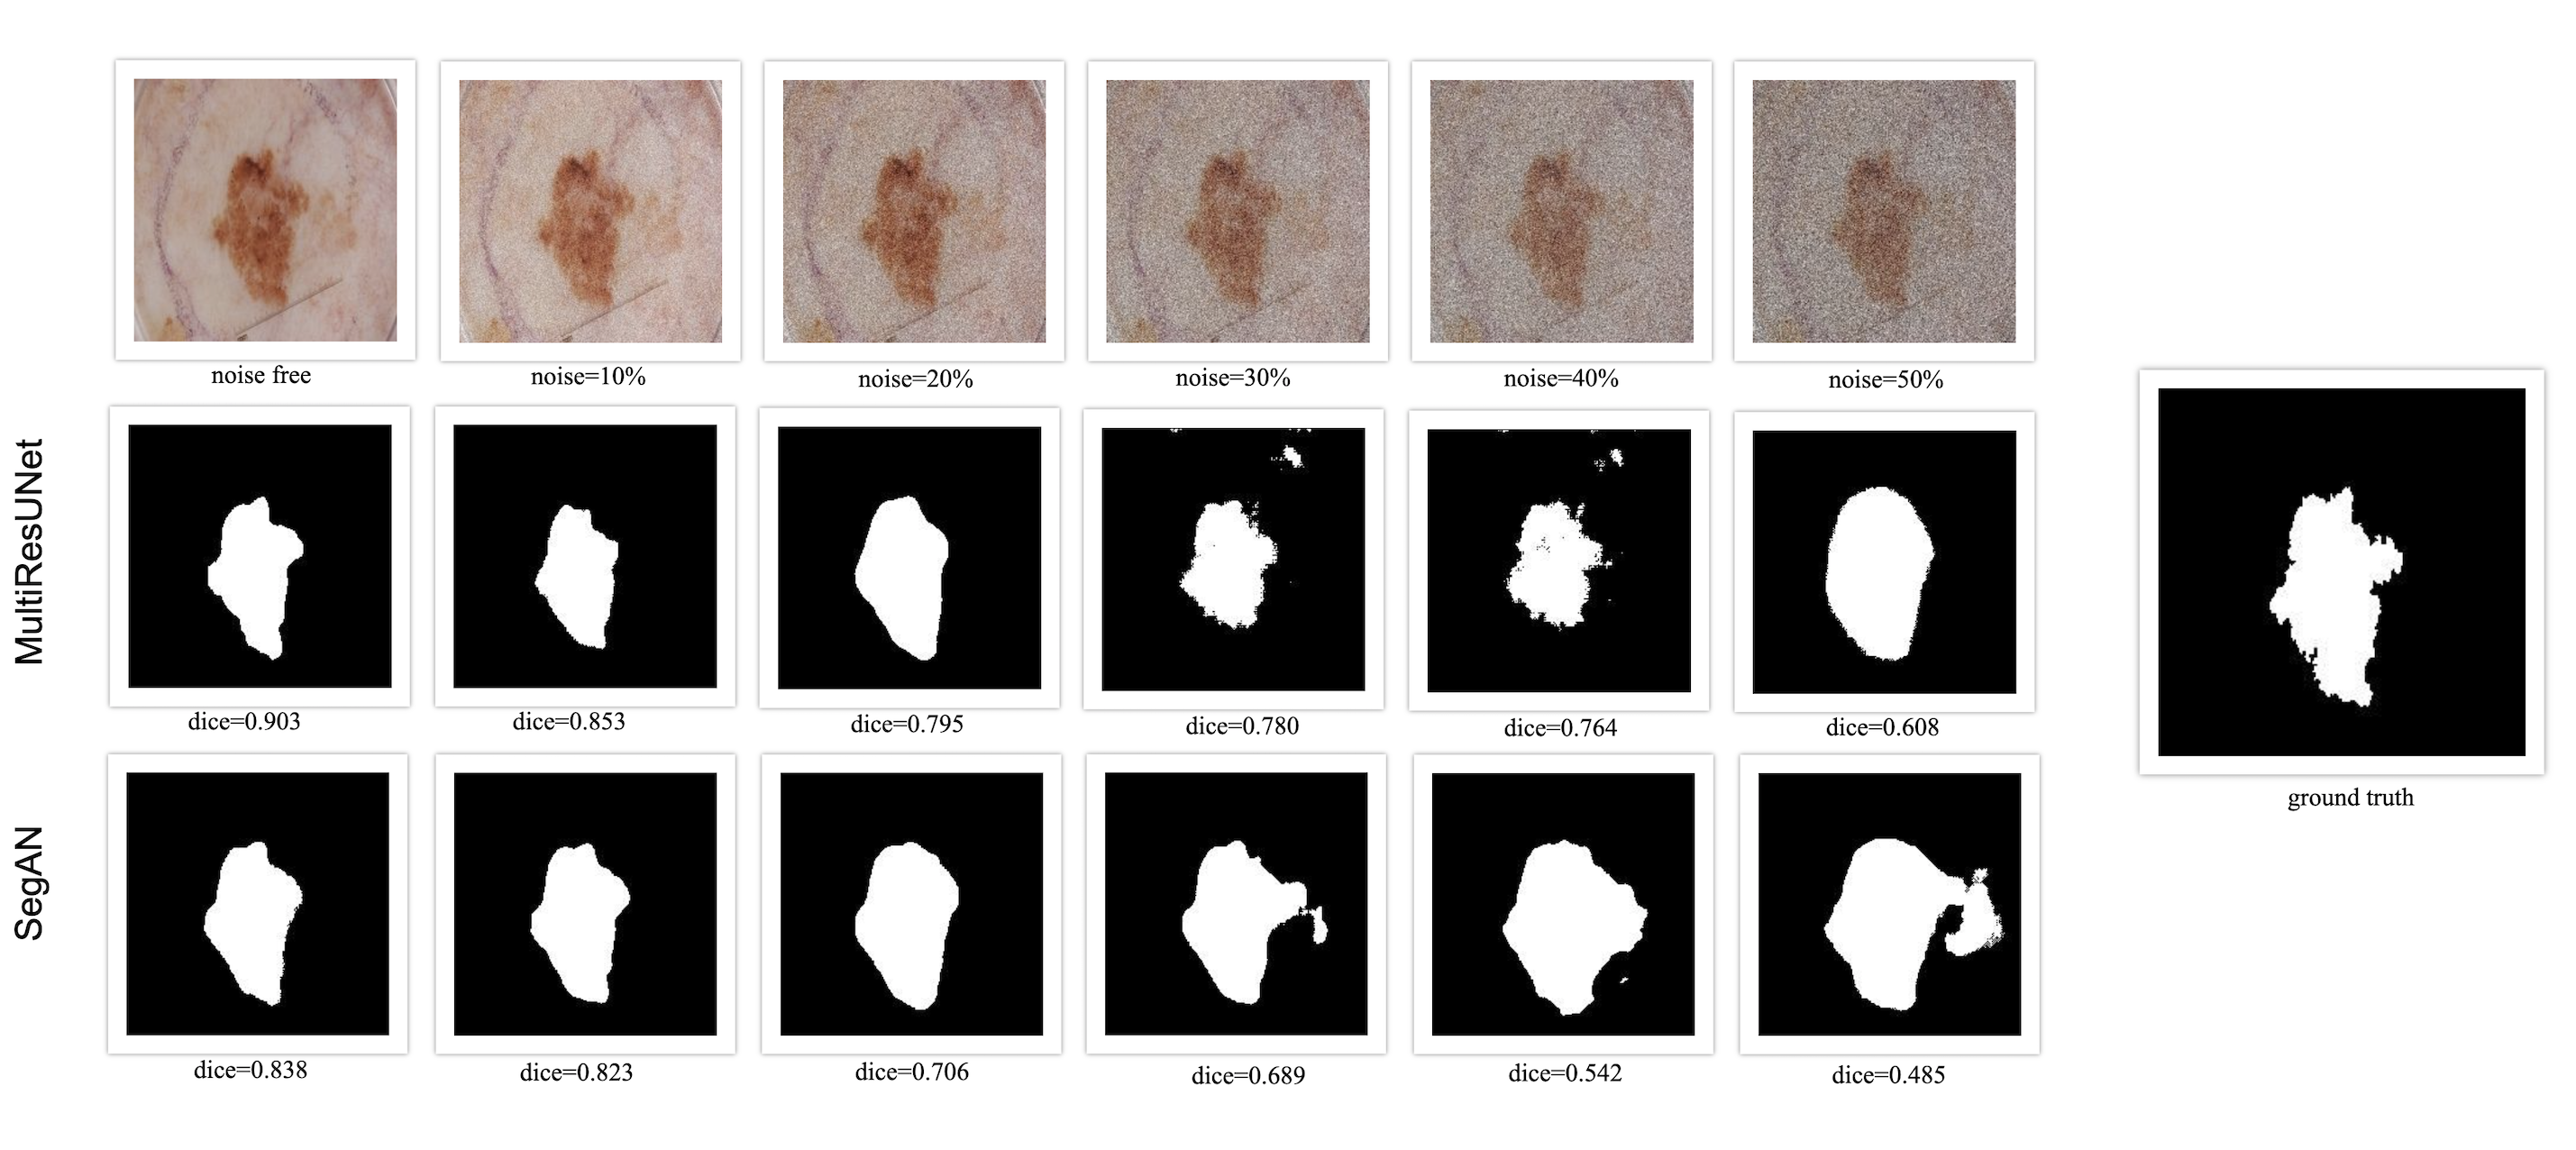
\includegraphics[width=1\columnwidth]{05-results/figures/extended_results_sample_unet_over_gan.png}}
    \caption{Dice results of the same image for the all networks at different Gaussian noises. The images in a column from top to bottom show the input, results of MultiResUnet, SegAN, and U-Net respectively. U-Net has better results}
    \label{figure:all-noises-with-results-dice-multiresunet-over-segan}
\end{figure}



    Although it is not possible to create a model that fit all dataset, it is the main objective to present a model that best generalizes them
    Figures ~\ref{figure:all-noises-with-results-dice-segan-over-multiresunet} and Figure ~\ref{figure:all-noises-with-results-dice-multiresunet-over-segan}
    are the outputs obtained by evaluating 2 pictures with two models in different levels of noises.
    While SegAN give more successful results for the image in Figure ~\ref{figure:all-noises-with-results-dice-segan-over-multiresunet},
    MultiResUNet is more successful in the image of Figure ~\ref{figure:all-noises-with-results-dice-multiresunet-over-segan}.
    As can be seen from that comparision, there is no precise superiority of the models to each other for certain data.

